% ==============================================================================================
\chapter{Moving load on an elastic halfspace} \label{ch:moving_load_halfspace}
% ==============================================================================================

% ----------------------------------------------------------------------------------------------
\section{Introduction}
% ----------------------------------------------------------------------------------------------
This benchmark compares the STEM numerical solution against the analytical solution,
for a moving load travelling on an elastic halfspace.

The analytical solution is presented in~\cite{Liao_Teng_Yeh_2005}.
The analytical solution provides closed-form expressions for the vertical displacement along the surface of the
halfspace, enabling a direct time-history comparison against the numerical model.

% ----------------------------------------------------------------------------------------------
\section{Model Description}
% ----------------------------------------------------------------------------------------------

% ..............................................................................................
\subsection{Geometry, mesh and loading}
% ..............................................................................................
The soil domain is modelled as a three-dimensional block representing the halfspace, with the following dimensions:
height \qty{10}{\meter}, width \qty{10}{\meter} and length \qty{20}{\meter}.
The soil is discretised with second-order tetrahedral elements, using an average element size of \qty{0.10}{\meter}.
An overview of the geometry and mesh adopted for the analysis is shown in
Figure~\ref{fig:one_dim_wave_mesh}.

The moving load is modelled as a vertical point load travelling along the z-direction at a constant speed of
\qty{40}{\meter\per\second}.
The load has a magnitude of \qty{1000}{\kilo\newton}.

The nodes at the sides of the soil have absorbing boundaries at the free ends, and with fixed boundary conditions
on the perpendicular plane along the axis of symmetry.
At the bottom the soil is assumed to be fixed.


\begin{figure}
	\centering
	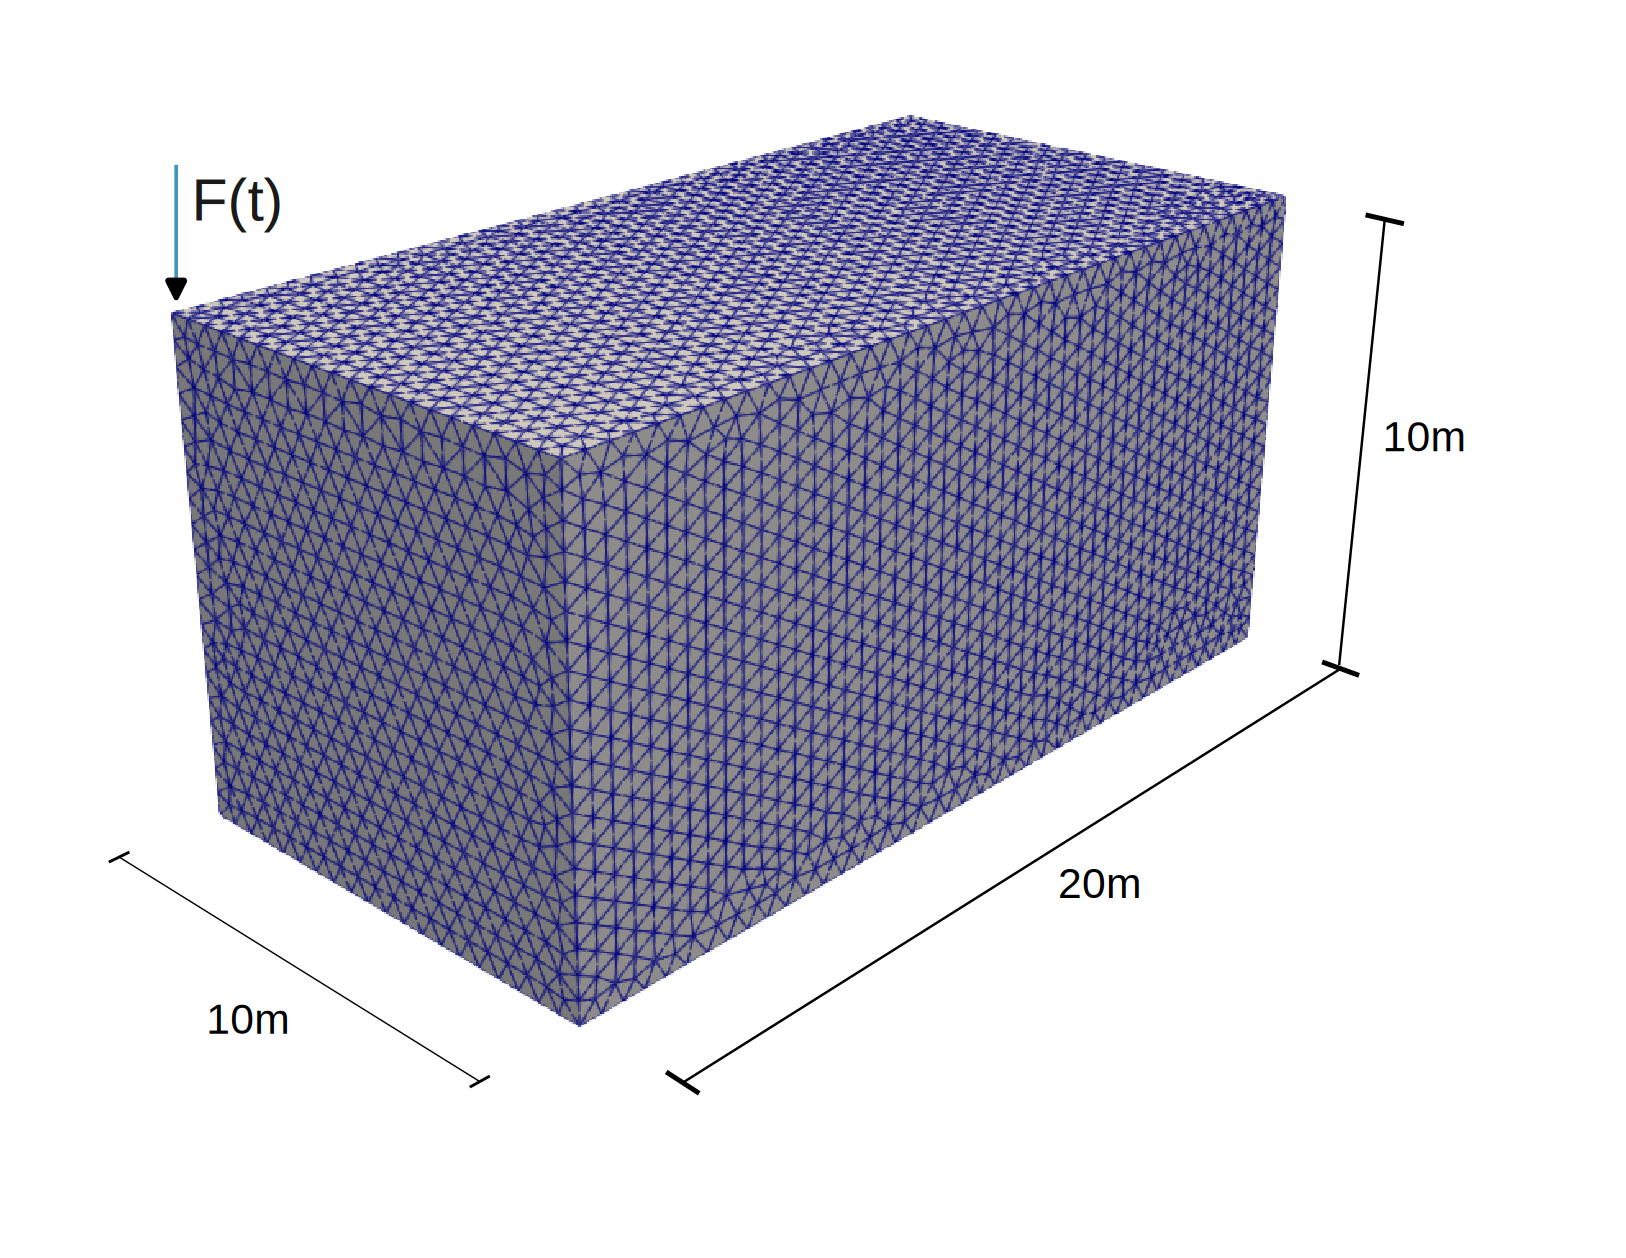
\includegraphics[width=0.75\textwidth]{moving_load/mesh.pdf}
	\caption{Geometry, mesh and boundary conditions adopted for the one-dimensional
	wave propagation benchmark.}
	\label{fig:one_dim_wave_mesh}
\end{figure}

% ..............................................................................................
\subsection{Materials and numerical parameters}
% ..............................................................................................
The soil is modelled as a one-phase continuum with a linear elastic constitutive law, with the
following parameters:

\begin{itemize}[noitemsep,topsep=0pt,parsep=0pt,partopsep=0pt]
	\item Young's modulus: \qty{50}{\mega\pascal},
	\item Poisson ratio: \qty{0.3}{},
	\item Solid density: \qty{2700}{\kilogram\per\meter\cubed},
	\item Porosity: 0.3.
\end{itemize}


Material damping is included via Rayleigh damping, with parameters that provide a damping ratio of
\qty{0.5}{\percent} at \qty{1}{\hertz} and \qty{80}{\hertz}.

The dynamic analysis is performed over a \qty{1}{\second} time window, with a time step of \qty{0.001}{\second}.
The system of equations is solved using the Newmark time integration~\cite{Newmark_1959} scheme with
parameters $\beta = 0.25$ and $\gamma = 0.5$.


% ----------------------------------------------------------------------------------------------
\section{Results}
% ----------------------------------------------------------------------------------------------
Figure~\ref{fig:one_dim_wave_results} presents the time histories of the
vertical velocity at three points located at: \qty{2.5}{\meter}, \qty{5}{\meter} and \qty{7.5}{\meter}
along the height of the column.
The figure compares the numerical STEM results against the analytical solution of the one-dimensional wave equation.

The arrival times of the incident and reflected waves at the observation point match closely between the numerical
and analytical solutions.
The amplitudes of the displacement and velocity pulses also show very good agreement, with small differences
attributable to the introduced material and numerical damping.

\begin{figure}[h]
	\centering
	\includegraphics[width=0.8\textwidth]{one_dim_wave_prop/time_history.pdf}
	\caption{Comparison of the vertical velocity time histories at three points located at:
    (a) \qty{2.5}{\meter}, (b) \qty{5}{\meter} and (c) \qty{7.5}{\meter}
	along the column height.}
	\label{fig:one_dim_wave_results}
\end{figure}

